\chapter{Analyse}

\section{Analyse des besoins}
% auteur : Rime
% relu : Fabien, Clément, Florian, Quentin

L’objectif initial était de réaliser un site communautaire, permettant à ses utilisateurs de proposer des services entre eux par l’échange d'une monnaie libre a travers un site épuré et agréable. 
Il a été nécessaire que l’on se réunisse plusieurs fois, afin de donner forme a ce projet, d’en dessiner les contours, de définir les tenants et les aboutissants. 
En effet, il était primordial de savoir exactement ce que ce site doit apporter. En quoi est-il intéressant~? A qui s’adresse-t-il en particulier~? Que propose-t-il de plus ou de différent par rapport aux sites existants~? Pourquoi, in fine, l’utilisation d’une monnaie libre~? 

Ce n’est que par cette analyse préalable, que nous avons pu identifier correctement les tâches à réaliser, les limites de notre projet et les éventuelles améliorations futures, dans une perspective d’évolution.

La première étape, s’est portée plus sur le fond que sur la forme ou la technicité. Il s’agissait de se donner un maximum d’idées sur ce que le site devait proposer. 
Vis à vis de l’objectif initial, il paraissait important de spécifier au mieux les services auxquels se rattache notre projet. C’est à dire, ce qu’il permettait de faire pour ses utilisateurs. Pour nous il était intéressant qu’un utilisateur puisse à la fois bénéficier de services et/ou en proposer. L’utilisateur de notre site devait donc avoir la possibilité, à sa guise, d’être un producteur et/ou un consommateur de services. Il devait être maître, non seulement, du choix du service qu’il désire (évident) mais aussi du type et de la hauteur de sa rétribution pour le service qu’il proposerait. 

Il apparu assez évident que les types d’échanges se porteraient essentiellement sur des services à la personne, d’aide et de partage (type covoiturage, couchsurfing et troc). 
À priori, un site comme le Bon coin (voir \cite{bc}) le permettait déjà. Cependant, c’est là que l’idée de monnaie libre nous distinguait de l’existant. Jusqu’à présent, le principal modèle de rétribution d’un service était celui de l’argent. À ce modèle encore largement prédominant, apparaissait de plus en plus des réponses de substitution. La monnaie libre permettrait de générer des échanges de services entre individus sans argent réel. Ce projet s’inscrit donc dans une perspective d’utilité sociale par la proposition d’un modèle alternatif d’échange de services. 

\section{Analyse de l'existant}
% auteur : Fabien
% relu : Clément, Florian

Des SELs (Système d'Echange Local) existent dans plusieurs régions de France sous forme de «~réunions~» où les différents usagers peuvent communiquer et échanger leurs services. 
Ce type d'échanges ne semble pas au goût du jour, en effet, l'Informatique a pris une place prépondérante dans notre système, dans notre mode de vie.
L'idée de proposer ces échanges par le biais de l'outil informatique est donc d'un enjeu important car elle en permet une adaptation moderne et pratique.
Un SEL en ligne existait déjà, «~Flowplace~» (voir figure \ref{fig:flowplace}), mais il ne semblait pas tout à fait effectif, il a, semble-t-il, d'ailleurs fermé à ce jour.
Nous étions donc libre d'imaginer comme nous le souhaitions notre site.

\begin{figure}[ht]
\centering
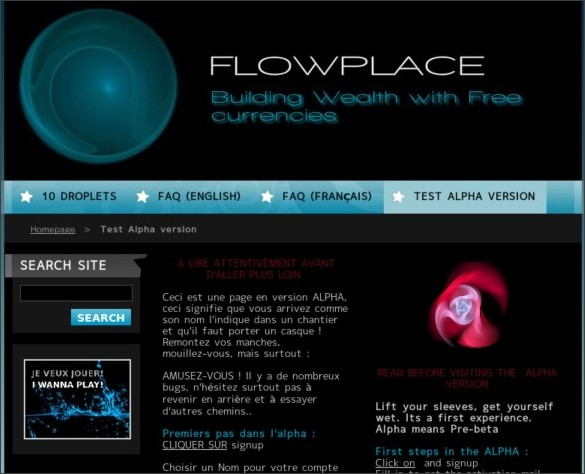
\includegraphics[width=0.9\textwidth]{flowplace}
\caption{Flowplace}
\label{fig:flowplace}
\end{figure}

\subsection{Analyse préalable}
% auteur : Rime
% relu par : Fabien, Clément, Florian

Lors de l'analyse, le référentiel utilisé fut le point de vue de l’utilisateur de notre site. 
Il fut décidé d'identifier un utilisateur par son nom, son prénom et son pseudo.
Il fut également choisi d'attribué à l'utilisateur une grandeur quantifiable nommée Karma, en référence à l’ensemble des bonnes et mauvaise actions qu’il aura réalisé au cours de son activité sur le site. Cette grandeur peut s'apparenter à une note de satisfaction, attribuée par les autres utilisateurs auxquels il aurait rendu service.
L'idée de proposer des «~missions~» aux utilisateurs fut aussi abordée, mais ne fut finalement pas retenue pour le projet final. Ces «~missions~» devaient être un ensemble des services qu'un utilisateur devait effectuer ou proposer, recevant en échange des récompenses monétaires et/ou en karma.
Nous abordions également le thème de la «~monnaie~». Un utilisateur devait pouvoir choisir de «~payer~» ou de se faire «~payer~» dans la monnaie libre du site, complètement décorrélée de quelconque monnaie existante. Cela devait s'apparenter à une quantité de «~points~» qui permettrait l’échange de prestations entre utilisateurs. 

Au départ, un nouvel utilisateur devait posséder un Karma neutre et une quantité de monnaie qui pourraient fluctuer au cours de son activité intra-site.

Chaque utilisateur devait également être attaché à un compte unique. Ce compte enregistrerait les diverses transactions et calculerait dynamiquement le solde restant, à l'instar d'un compte bancaire.

L'idée de groupe fut également abordé. Chaque membre pouvaient faire partie d'un ou plusieurs groupes. 
À ces groupes devait également être rattachée une liste de services.

\section{Diagrammes de cas d'utilisation}
% auteur : Quentin
% relu : Clément

\subsection{Cas d'utilisation : Membre}

\begin{figure}[ht]
\centering
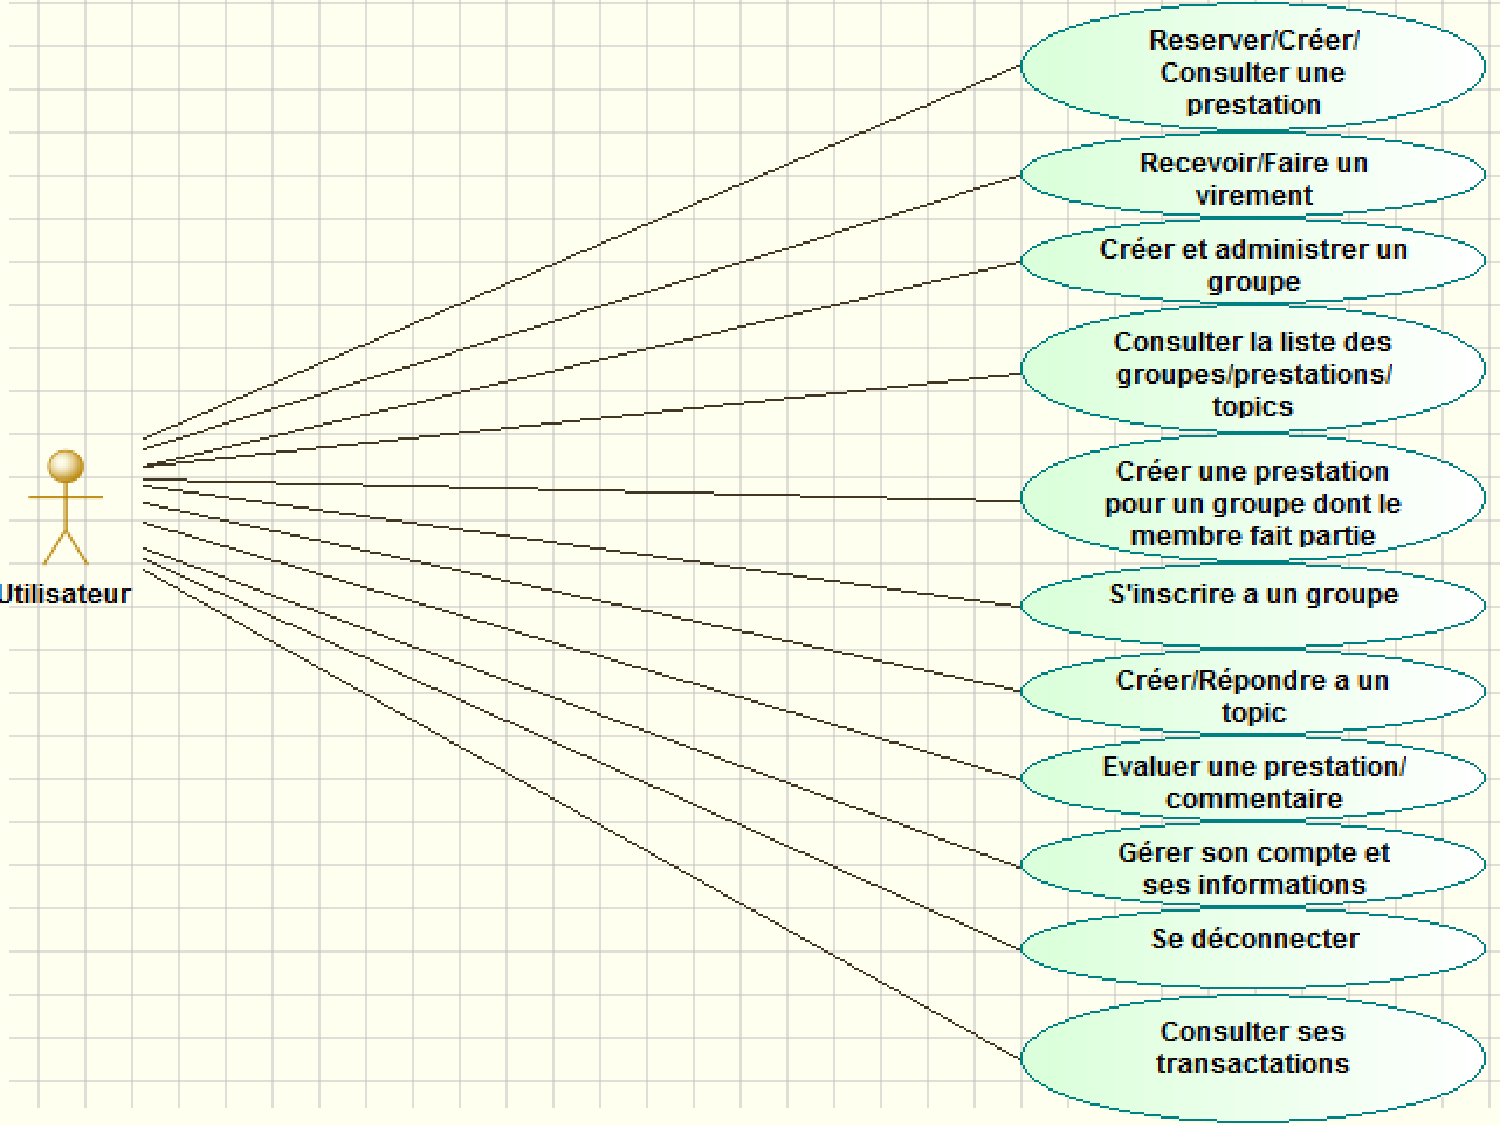
\includegraphics[width=0.9\textwidth]{UseCaseUtilisateur}
\caption{Diagramme de cas d'utilisation d'un utilisateur}
\label{fig:UseCaseUtilisateur}
\end{figure}

A la figure \ref{fig:UseCaseUtilisateur} nous pouvons constater les actions qui sont disponibles pour un membre.
Un membre peut donc réserver, créer ou consulter une prestation, faire ou recevoir un virement, créer et administrer un groupe de membres, consulter la liste des groupes, prestations et topics, créer une prestation pour un groupe dont le membre fait partie, s'inscrire à un groupe, créer et répondre à un topic, évaluer un topic ou une prestation, gérer son compte et ses informations et, enfin, se déconnecter.

\subsection{Cas d'utilisation : Modérateur}

\begin{figure}[h]
\centering
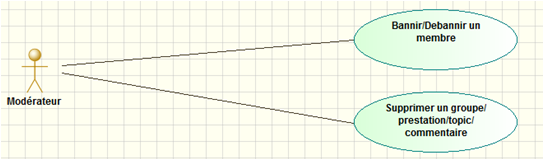
\includegraphics[width=0.9\textwidth]{UseCaseModerateur}
\caption{Diagramme de cas d'utilisation d'un modérateur}
\label{fig:UseCaseModerateur}
\end{figure}

A la figure \ref{fig:UseCaseModerateur} nous pouvons constater les actions qui sont disponibles pour un modérateur.
Un modérateur a pour responsabilité de veiller à ce que les services soient corrects, qu'il n'y ait pas d'abus au niveau des interactions entre les utilisateurs.
Pour mener cette tâche à bien, un modérateur peut bannir ou débannir un membre, supprimer un groupe, une prestation ou encore un topic.

\section{Diagrammes de classes}

\subsection{Diagramme de classe prévisionnel}
% auteur : Oualid, Quentin
% relu par : Clément, Florian

\begin{figure}[ht]
\centering
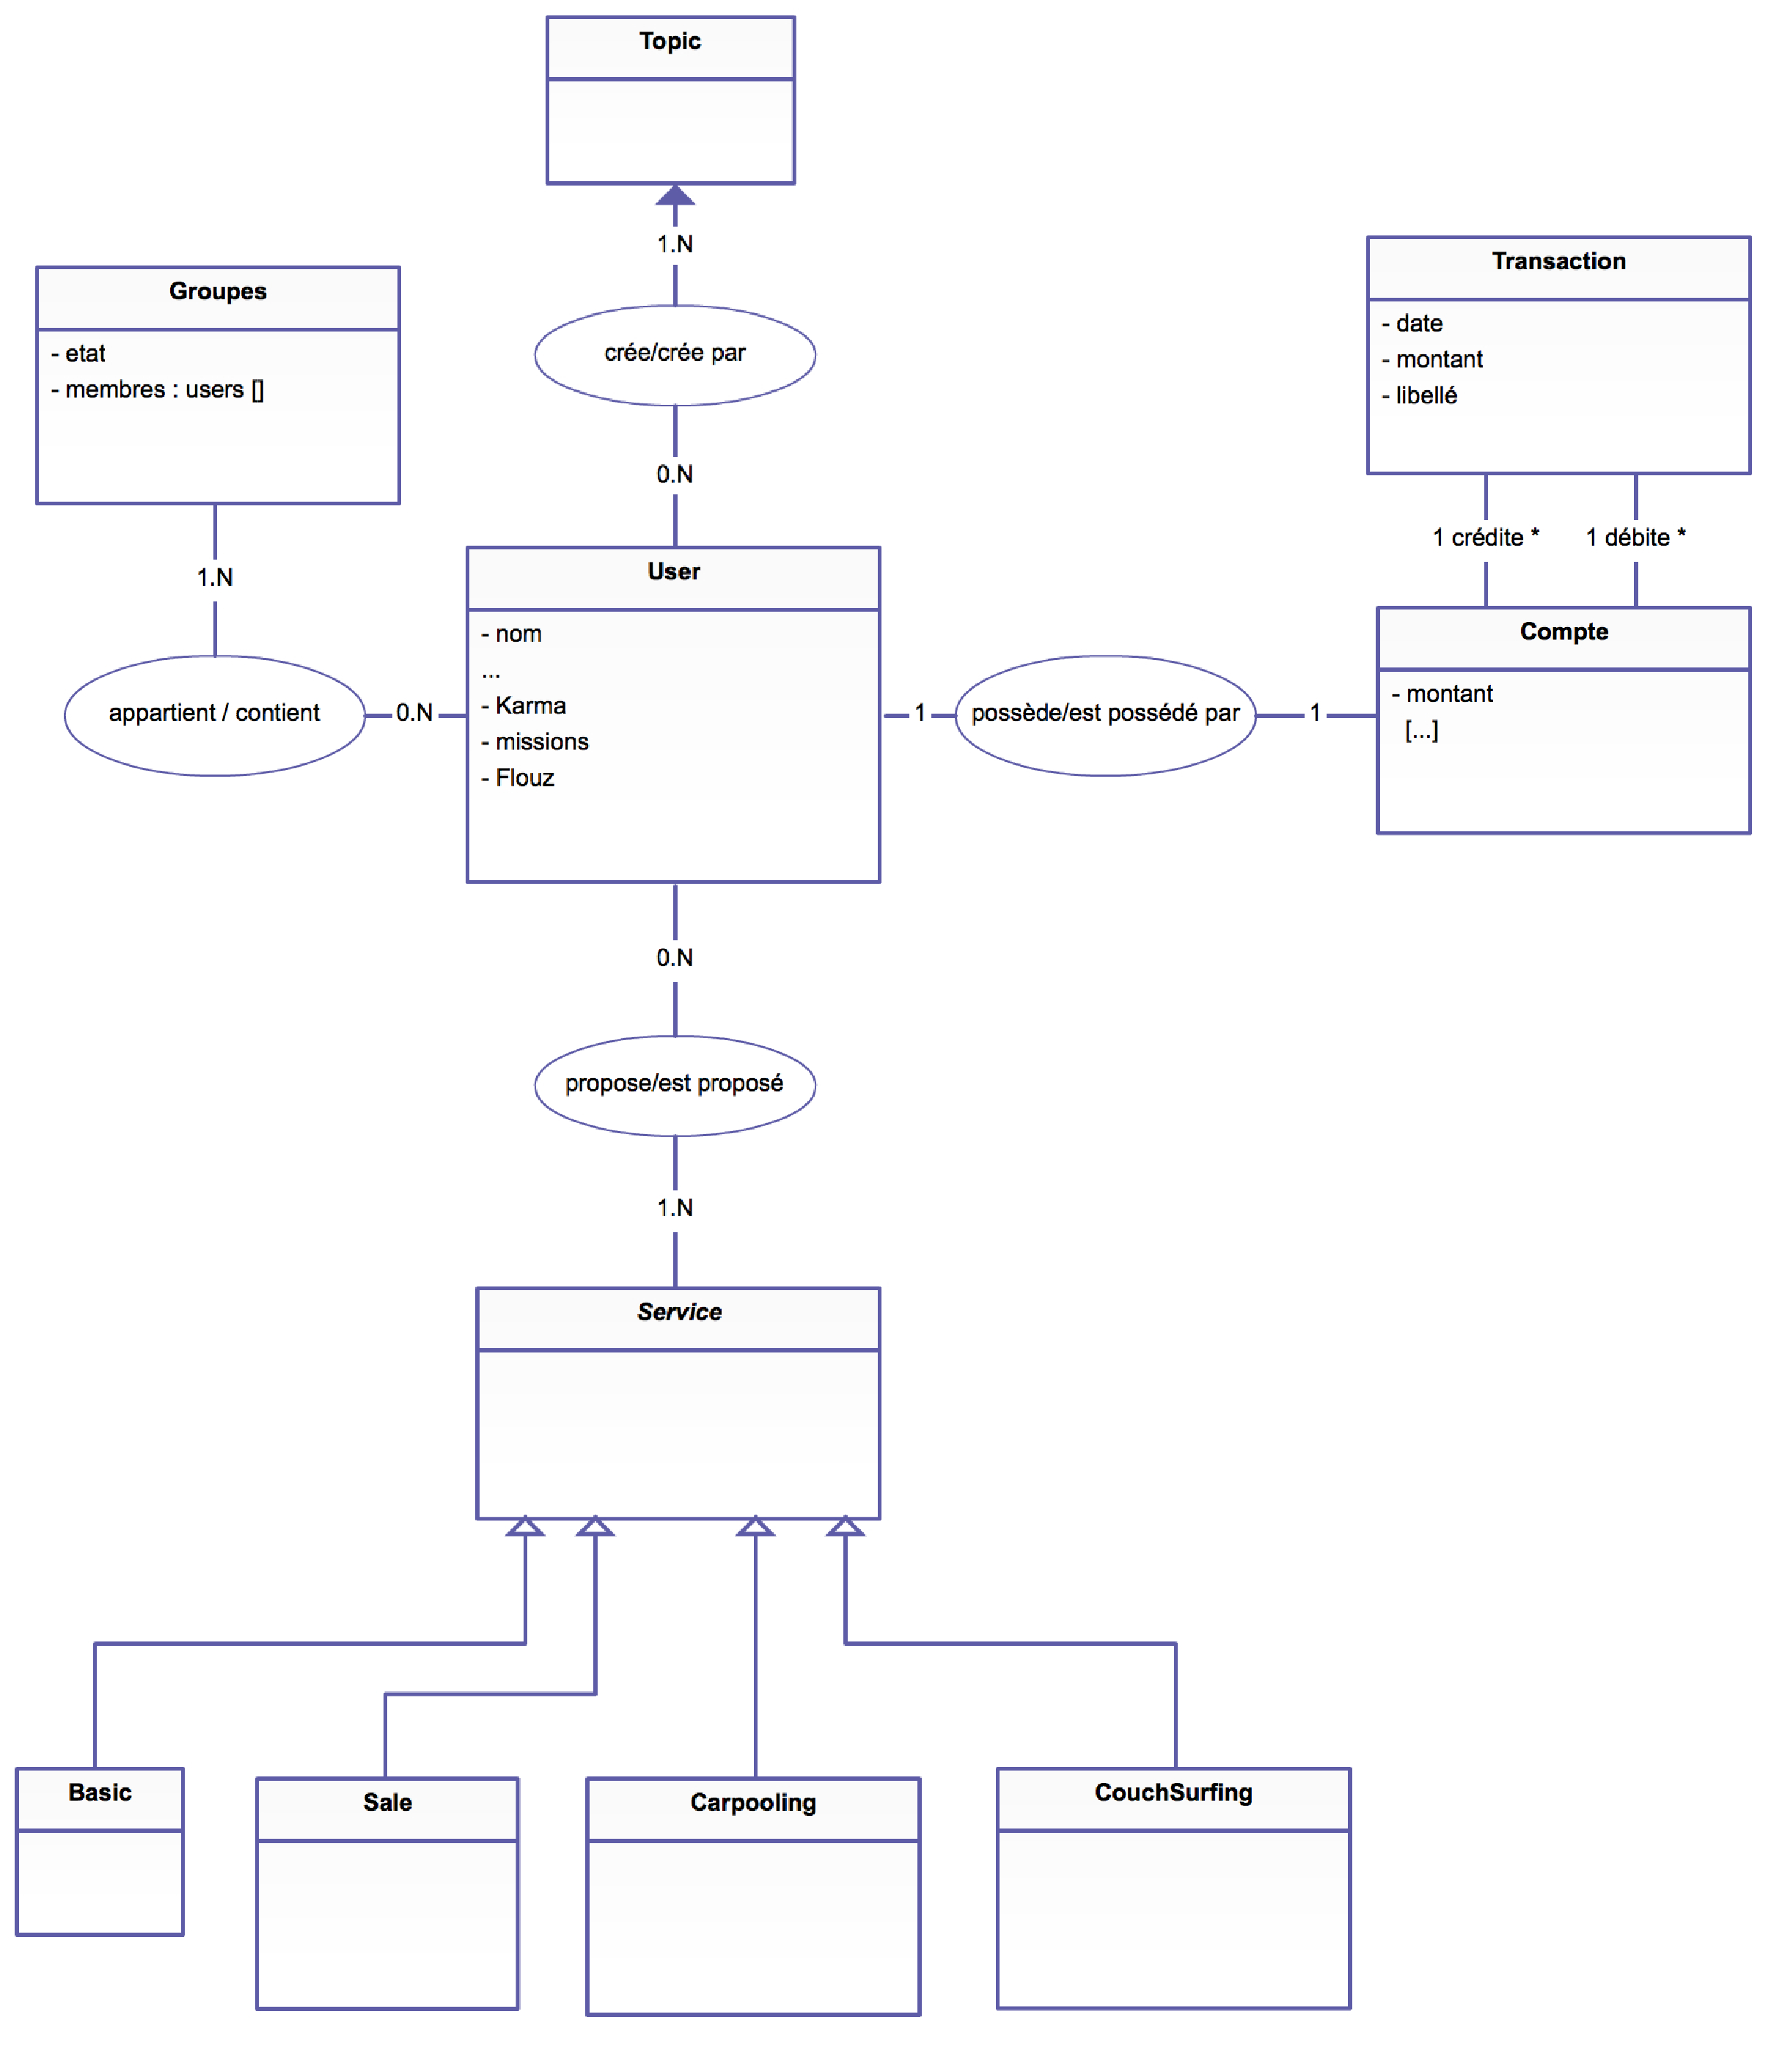
\includegraphics[width=0.9\textwidth]{diagramme-classe-previsionnel2}
\caption{Diagramme de classe prévisionnel}
\label{fig:diagramme-classe-previsionnel2}
\end{figure}

La figure \ref{fig:diagramme-classe-previsionnel2} représente la modélisation du système au niveau des classes que nous avions prévues avant de commencer à coder. 
Il a ensuite bien évolué...

\subsection{Diagramme de classe final}
% auteur : Oualid, Quentin
% relu par : Florian, Clément
\begin{figure}[ht]
\centering
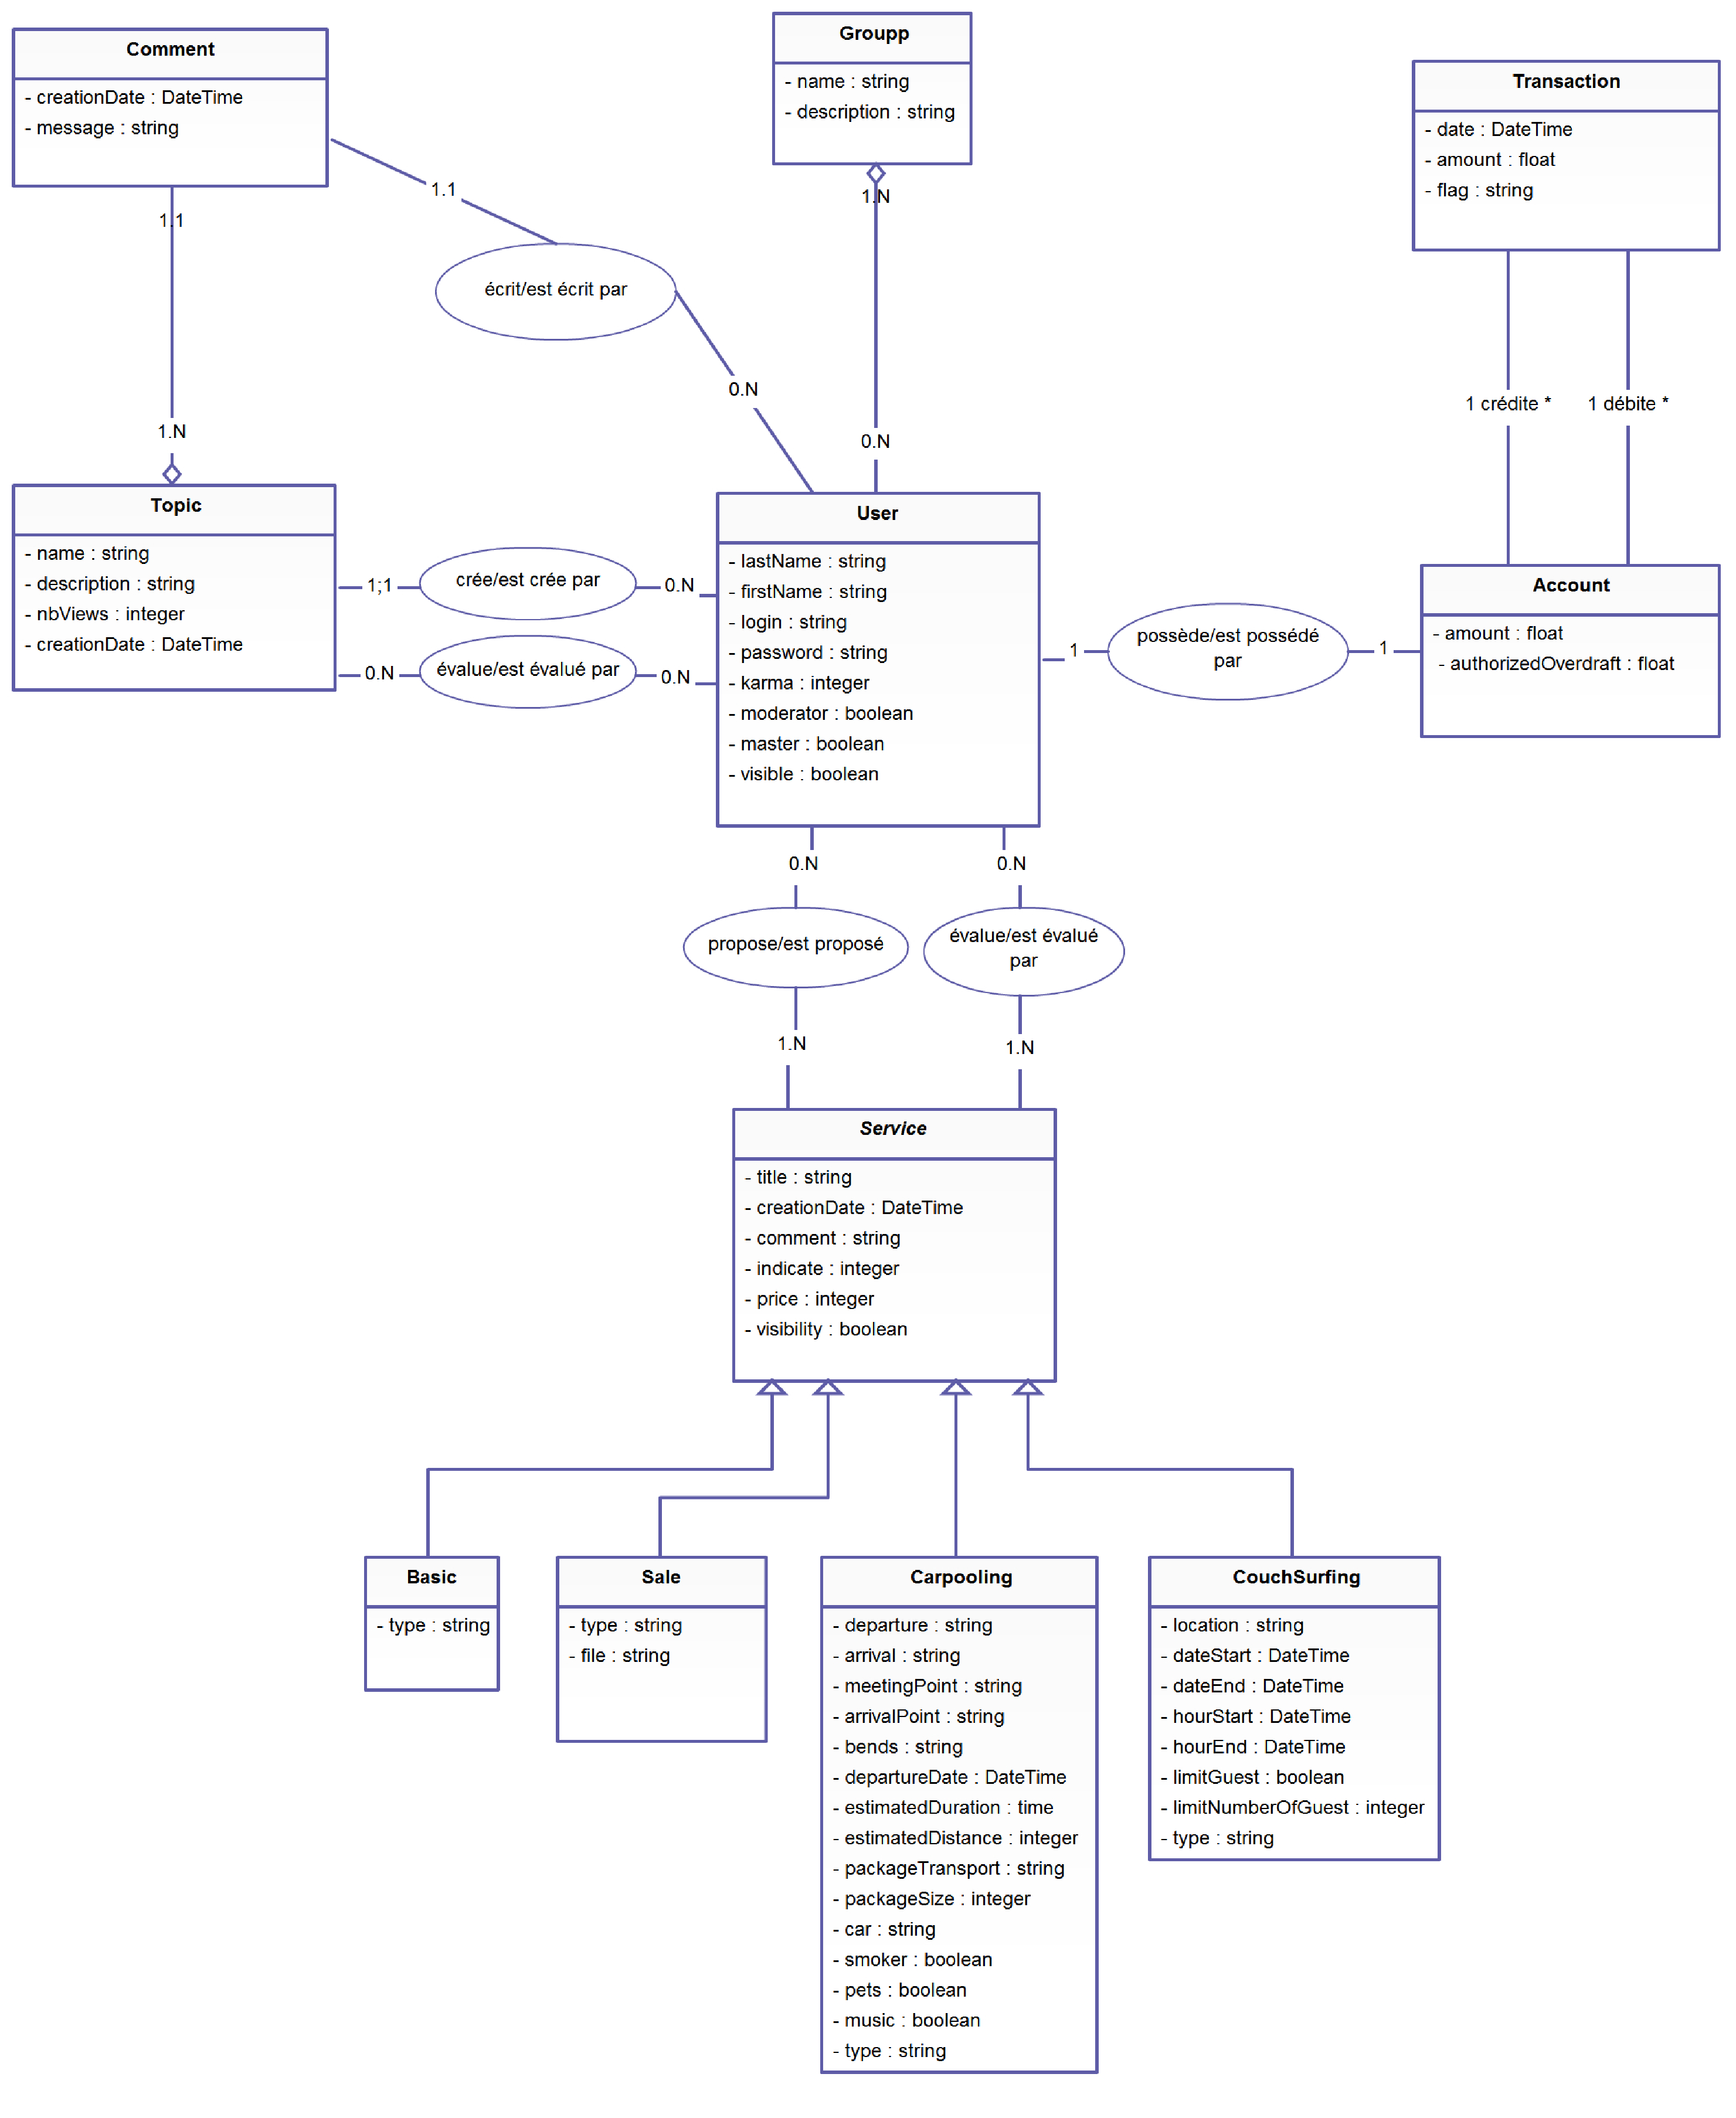
\includegraphics[width=1.0\textwidth]{diagramme-classe-final}
\caption{Diagramme de classe final}
\label{fig:diagramme-classe-final}
\end{figure}

Le diagramme qui apparaît à la figure \ref{fig:diagramme-classe-final} représente nos classes d'un point de vue conceptuel. C'est le diagramme de classe final, il implémente actuellement notre système.

% auteur : Rime
% relu : Fabien, Florian, Clément

Notre diagramme prévisionnel a évolué vers son état final en ce diagramme. 
Cette fois-ci les services se divisent en quatre grandes catégories :
\begin{description}
\item [Couchsurfing] qui correspond à trouver/proposer un logement temporaire~;
\item [Covoiturage] qui permet un déplacement à plusieurs partageant ainsi les coûts inhérents au voyage~; 
\item [Ventes] qui, à l’instar de sites comme Le Bon Coin ou encore Ebay, permet des échanges d'objets~; 
\item [Basique] qui correspond à tout ce qui est autre que les trois catégories pré-citées.
\end{description}

La possibilité pour chaque utilisateur d’utiliser un forum afin de favoriser le lien social et d’expliciter éventuellement au mieux sa demande et/ou proposition. 
Le karma quant à lui est toujours une quantité qui fluctue en fonction des évaluations des autres utilisateurs ayant bénéficiés du service fourni. 
De plus, chaque classe a été définie par un certain nombre d’attributs qui sont plus précis que ceux du diagramme prévisionnel. Ceux-ci sont commentés plus spécifiquement dans la section en rapport avec les bundles.

